%!TEX root = ../../thesis.tex

\section{A frame is a generic function}
\label{chapter:limitations:framegeneric}

In this section, we provide example of what a frames might be. In all the experiment consider until now, we only considered the feedback and guidance frame which implies many constraint on the interaction protocol and the abilities of the robot. For example, the user should deliver feedback after one action of the robot, this simple interaction already requires to implement a turn taking social behavior in the robot, but also means that the user is able to see know when one action has been executed by the robot. On the other side, the robot need to interpret the signal from the user with respect to many objectives, and in our scenarios, this requires the robot to know the optimal plan in each state and for every task hypothesis. This kind of constraints are usual in BCI scenario, where it is still difficult to extract information continuously from ErrP EEG signals and where the task to be execute is often discrete and of low complexity such that it is easy for our agent to compute the optimal policies for each task. In the following of this section we describe a few frame that may be considered for extending this work to more real world robotic scenario.

\subsection{A task is not always a fixed target}

In this thesis, we only considered task which where represented as a sparse reward function represented in the MDP framework. However there is explicit reason of being limited to this choice, and especially the fact that one task represents a particular state of the world. A task may be an endless repetition of action such as for a robot in an assembly line that should be taught to assemble a given object again and again. Or a robot that should patrol around houses. 

For our feedback and guidance frame, as soon as the policies associated to each task can be provided to the robot, our algorithm scan be applied. We present in Figure~\ref{fig:gridwolrdgenericframes} two examples where policies are easy to define but are not always possible to derive in a simple MDP representation.

The policy of Figure~\ref{fig:gridwolrdgenericframesaround} consist of following the external wall of the grid world in a clockwise direction. This policy can not be derived from a state based reward function. Similarly in Figure~\ref{fig:gridwolrdgenericframesaround}, the policy consist of a endless looping trajectory, which can not be described by a reward function on our 9 states space. This kind of policies are rather easy to define by hand or by randomly generating them on a computer. 

\begin{figure}[!htbp]
\centering
    \begin{subfigure}[b]{0.49\columnwidth}
        \centering
        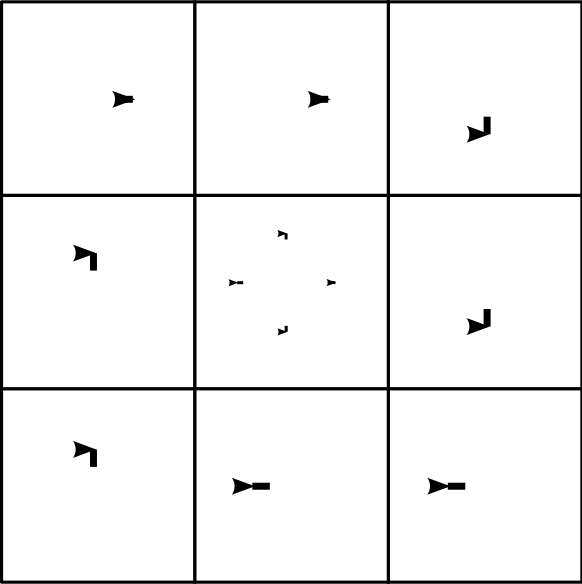
\includegraphics[width=0.8\columnwidth]{\visualspdf/frame/gridworld_around.pdf}
        \caption{W}
        \label{fig:gridwolrdgenericframesaround}
    \end{subfigure}
    \begin{subfigure}[b]{0.49\columnwidth}
        \centering
        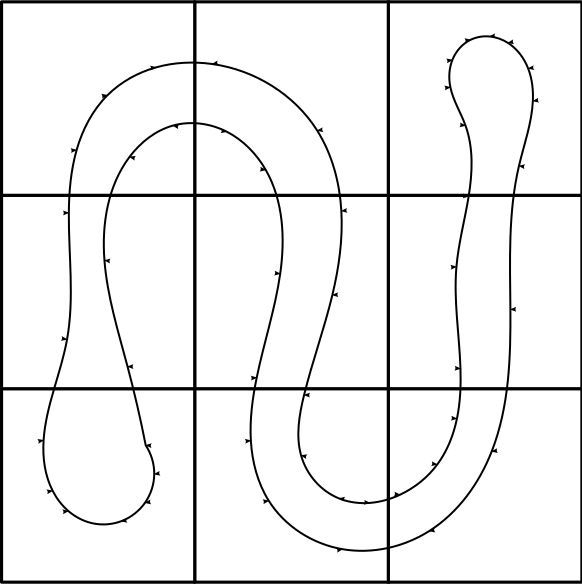
\includegraphics[width=0.8\columnwidth]{\visualspdf/frame/gridworld_loop.pdf}
        \caption{W}
        \label{fig:gridwolrdgenericframesloop}
    \end{subfigure}
\caption{Two examples of desired agent behavior that are harder to define in terms of rewards function.}
\label{fig:gridwolrdgenericframes}
\end{figure}

We note that it is always possible to represent the problems such that a fixed reward function allows to infer the policies of Figure~\ref{fig:gridwolrdgenericframesaround}~and~\ref{fig:gridwolrdgenericframesloop}. For Figure~\ref{fig:gridwolrdgenericframesaround} defining a reward function on the state-action space would be enough. For Figure~\ref{fig:gridwolrdgenericframesloop}, it is more challenging as the Markov properties are not respected, indeed it is necessary to known the previous position of the agent to predict its future position. Therefore the representation of the agent state should include the previous position of the agent, which increases the state space from 9 states to 81 states.

\subsection{No need for planning skills}

We provide an example of interaction frame where the agent do not need to know the optimal policy to interpret a signal with respect to a particular objective. In this frame, the goal of the robot is to locate one object or find one particular position in a 2D space. The teacher provide indication on the absolute direction of such object with respect to the agent position. As an example, we consider a teacher that indicates the cardinal direction of the object, i.e. the message to the robot is: \emph{``the object is North (South, West or East) with respect to your position''}.

We illustrate this frame in Figure~\ref{fig:cardinalframe}. The choice of the cardinal direction to send to the agent is modeled by a probabilistic models, where the probability of one cardinal direction is proportional to the angle between the target-agent direction and the cardinal direction considered.

\begin{figure}[!htbp]
    \centering
    
\includegraphics[width=0.8\columnwidth]{\visualspdf/frame/cardinal_frame.pdf}
    \caption{Example of the cardinal frame. The signal from the teacher indicates in which cardinal direction (N,S,W,E) the goal position or the object to reach is. There is a probabilistic model that describe the user behavior, such that the probability of generating a signal of meaning ``West'' is proportional to the angle between the agent position and the target position. This frame does not requires the agent to know how to reach the target position, but only its own position with respect to that goal.}
    \label{fig:cardinalframe}
\end{figure}

We defined as $\varphi_N$ the angle between the target-agent direction and the North cardinal direction, and respectively $\varphi_S$, $\varphi_W$, and $\varphi_E$ the angles with respect to the South, West, and East directions. The probability of that the user refers to the North cardinal direction is defined as follows:

\begin{equation}
    p(l^f = \emph{north}~|~\varphi_N) = 
    \begin{cases}
    (1 - \frac{2 \varphi_N}{\pi}) (1-\alpha) & if~\varphi_N < \frac{\pi}{2}\\
        \frac{\alpha}{K}  & \text{otherwise}\\
   \end{cases}
   \label{eq:cardinalframe}
\end{equation}
with $K$ the number of cardinal direction that do not satisfies the condition $\varphi_N < \frac{\pi}{2}$, which means K can take value of 2 or 3 only. $\alpha$ is the error rate of the user. Finally, we consider unsigned angles only within the $[0, \pi]$ intervals only, meaning that angles of $\frac{-\pi}{2}$ or $\frac{3\pi}{2}$ are taken as $\frac{\pi}{2}$. The same equation applies for all cardinal direction and should maintain the following properties $\sum_{c \in \{N,S,E,W\}} p(l^f = c |\varphi_c) = 1$.

In practice, if we consider our visual representation of Figure~\ref{fig:cardinalframe}, we obtain the following angle measurements: $\varphi_N = \frac{9\pi}{22}$, $\varphi_S = \frac{13\pi}{22}$, $\varphi_W = \frac{20\pi}{22}$, and $\varphi_E = \frac{\pi}{11}$. In that case $K = 2$. If we consider $\alpha = 0$, we obtain the following probabilities values: $p(l^f = \emph{north}~|~\varphi_N) = 0.18$, $p(l^f = \emph{south}~|~\varphi_S) = 0$, $p(l^f = \emph{west}~|~\varphi_W) = 0$, and $p(l^f = \emph{east}~|~\varphi_E) = 0.82$, which we represent as a vector $[0.18,0,0,0.82]$. If we account of some probability of errors from the teacher, taking for example $\alpha = 0.05$, we obtain the following vector of probability: $[0.17, 0.025, 0.025,0.78]$.

We will use this frame in our experiment of section~\ref{chapter:limitations:continuoushypothesis}. Note that the same frame can apply with different referential, instead of the cardinal direction, one could refer to the direction with respect the robot orientation, or with respect to the position of the human teacher in the room, etc.

\subsection{Asynchronous instructions}

The interaction between our users and our robot would be easier if the robot could act continuously and the human would provide instruction when he deemed necessary. For example, in our pick and place scenario of chapter~\ref{chapter:lfui} it is boring for the user to provide feedback after each movement of the robot, it would be easier to wait the robot has displaced a cube to an other location. In addition, in some domains, the frequency of action is to high to afford waiting for a feedback signal between each action. Either the action would be so small that the user would not be able to judge the action, either the interaction flow would be dramatically affected by the many pauses in the task execution.

To allow for continuous operation of the robot, asynchronous delivery of signals should be accepted. A potential avenue is to consider a temporal function that distribute a signal event across some subset of previous robot events. This method has been used by Bradley Knox et al. in their TAMER framework \cite{knox2009interactively} using a data from a study of the distribution of human response times \cite{hockley1984analysis}.

\subsection{Including social clues}

As for tackling the problem of asynchronous instructions, information known to be true for most interaction scenario can be included in the frame definition.  Such as whether the human is looking at the scene or not, but also the presence of other persons in the room, or that some objects are hiding parts of the world to the human eye, etc.
